%Here you can see how to include an image in your document.


%Here is the command to refer to another element (section, figure, table, ...) in the document: \emph{As discussed in Section~\ref{sect:overview} and as shown in Figure~\ref{fig:metamodel}, ...}. Here is how to introduce a bibliographic citation~\cite{DAM}. Bibliographic references should be included in a \texttt{.bib} file. 

%Table generation is a bit complicated in Latex. You will soon become proficient, but to start you can rely on tools or external services. See for instance this \href{https://www.tablesgenerator.com}{https://www.tablesgenerator.com}. 
{\color{Blue}{\subsection{Product Perspective}}}
\setlength{\parskip}{0.5cm}
Data4Help is a system that involves two type of entities: Users and Third Parties. In order to keep the difference between the two entities sharper, the User will be provided with an application, instead the Third Party will have to interact with the system with a website. Another reason for choosing this division is that for a company is easier to have a website to work on their researches instead of an application that have to be downloaded on a smartphone.\\
On the other hand, for AutomatedSOS an application is the best way to interact with the User.\\
The reason for dividing the Data4Help and AutomateSOS applications is that only the ones who wants to benefit from the advantages of AutomatedSOS will have to download the application on their smartphone. In this way the two applications remain as easy as possible, only providing the required services.\\
In any case, Data4Help and AutomatedSOS are not independent, they have common characteristics especially for what concerns the types of data provided by the user to the system and the mechanism to manage monitoring devices associated to both the services. \\
To provide an overview of the main system elements and what will be specifically explained in further sections for Data4Help, the following block diagram can be useful:\\

\begin{figure}[H]
	\centering\setlength{\captionmargin}{0pt}%
	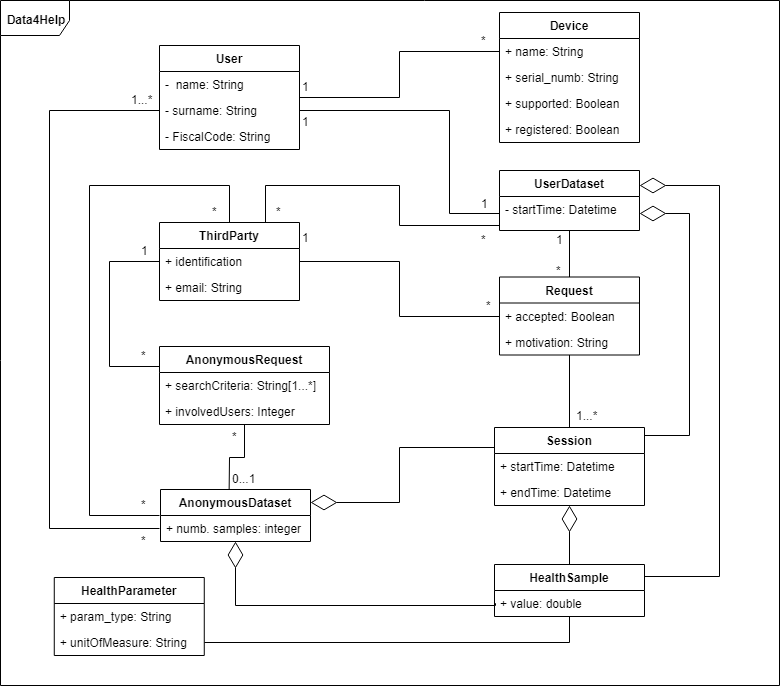
\includegraphics[scale=0.5]{Images/UML/D4H_class.png}
	\caption{Data4Help Class Diagram}
	\label{figure11}
\end{figure} 
\paragraph{}
As in the previous case a diagram can clarify the AutomatedSOS perspective:

\begin{figure}[H]
	\centering\setlength{\captionmargin}{0pt}%
	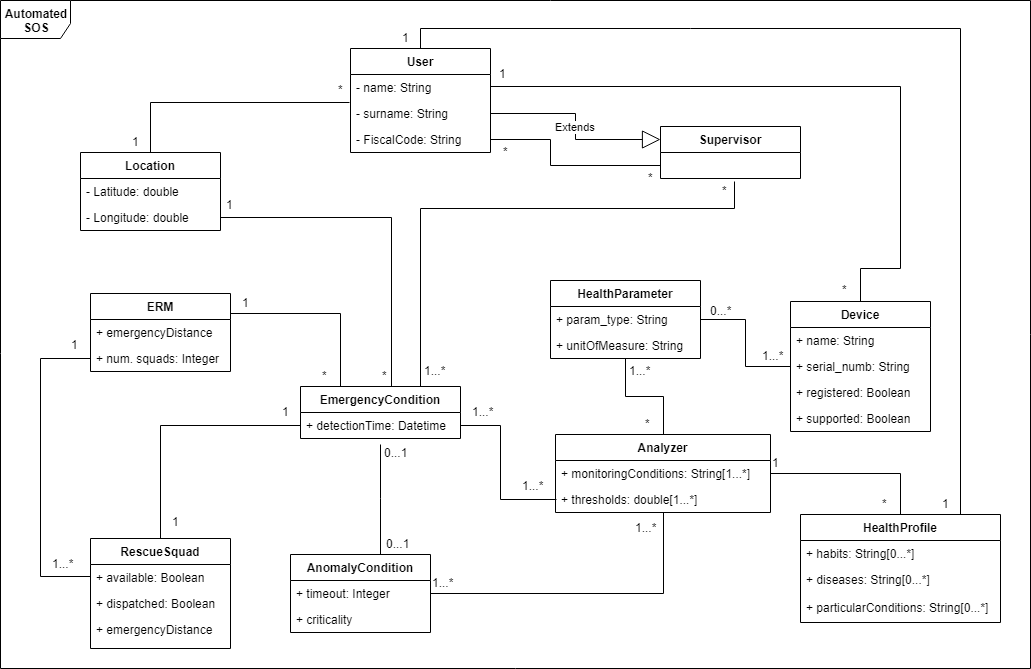
\includegraphics[scale=0.5]{Images/UML/ASOS_class.png}
	\caption{AutomatedSOS Class Diagram}
	\label{figure11}
\end{figure}



{\color{Blue}{\subsection{Product Functions}}}
{\color{Blue}{\subsubsection{Data4Help}}}
The main goal of Data4Help is to guarantee control on the health parameters of the users in order to give the possibility to third parties to obtain the data. Every user registered in Data4Help knows that his/her registered parameters could be used for market information, but also for helping researchers to discovers new treatments. This is made possible by providing two types of registration: the registration as a user and the registration as a third party.\\
There will be the possibility for the users to accept or deny personal requests from third parties, in this way there will be no privacy violations. On the other hand, the system will allow third parties to formulate anonymous requests. These are intended to not disclose the identity of the user, providing information of an heterogeneous set of users according to several requestor-specified search criteria. Unfortunately, it is trivial for a third party to trace back to sensitive information of a user providing restricting search parameters. After an attempt analysis, TrackMe evaluated a policy to prevent this possibility: in order to provide the result of an anonymous request to a third party, the involved users must be at least 1000. 
 %On the other hand, every request from the third party that comprehend at least 1000 of anonymous users will not require the consultation of every single user involved.\\
 %in order to control user’s parameters is possible to connect to the service various types of sensor devices.\\
 
\newpage
{\color{Blue}{\subsubsection{AutomatedSOS}}}
AutomatedSOS wants the users to feel safe. Provided the necessary sensor devices, the system guarantee a constant control on the health parameters. 
In order to minimize medical resource wasting, it is necessary for the system to discriminate carefully which conditions may lead to a fatality (e.g: heart attack) from those which can be simply false positive detections, uncareful behaviors of the person who is using the service, non-serious injuries or ambiguous observations. To this end, the system will be able to detect emergency and anomaly conditions.
%\begin{itemize}
	%\item \textit{Emergency Conditions}: unambiguous detections triggered by so-called critical events (e.g: heart attack)
	%\item \textit{Anomaly Conditions}: ambiguous detections that expect a reaction of the user and can be turned into emergencies under certain conditions
%\end{itemize}
%Every alteration that could possibly lead to an emergency is immediately notified to the user that could confirm the emergency condition or deny it. Alteration that are definitely sign of emergency lead immediately to an ambulance call.\\
Obviously, in order to guarantee that the number of false positives remains as low as possible, the user is required to give correct health information when he/she registers to the service. Furthermore the system will not allow a user to choose arbitrarily which set of sensor types will be used to monitor his/her health conditions. For each specific disease selected, there will be a set of specific sensor devices required.\\ 
The system will also provide the possibility to accept supervisors. This particular characters are AutomatedSOS users concepted to be supported by the system for giving assistance to other ones designated as supervised. Each time an AutomatedSOS users is in danger the system will be able to provide to the designated supervisor the necessary information. In this way, in case of emergency, there will be someone promptly informed.\\
As is known that it is not always possible to be monitored by the system, there is the possibility to notify the latter that it has to stop controlling the user parameters by turning off the service. The system also stops controlling them when the minimum required sensors are not available (maybe because they run out of battery), sending a notification to the user.  

{\color{Blue}{\subsubsection{Requirements}}}
\textbf{Data4Help}
\begin{itemize}
\item\textbf{[R1]:} The system must allow a registered user to associate a sensor device to the service
\item\textbf{[R2]:} Each user is uniquely identified by the system
\item\textbf{[R3]:} The system can acquire health data by specific sensors connected to the user's main device
\item\textbf{[R4]:} The system must be able to identify and certificate the reliability of each organization that wants to request user data
\item\textbf{[R5]:} Each registered organization that wants to access health data of specific users must be able to formulate a request providing information related to the purpose of the request.
\item\textbf{[R6]:} The system must notify each user of a third party request as soon as it is formulated, and allow him/her to accept or reject the request
\item\textbf{[R7]:} For each third party request the system should provide to the user information related to the requester and the purpose of the request
\item\textbf{[R8]:} Once a third party request is accepted by the user, the third party must have full access to the entire collection of data of the user
\item\textbf{[R9]:} Third parties must be able to request health data of groups of anonymous users, according to several criteria without being expressively authorized
\item\textbf{[R10]:} The system must prevent third parties to trace back to specific user information through anonymous requests
\end{itemize}
\paragraph{}
\textbf{AutomatedSOS}
\begin{itemize}
\item\textbf{[R11]:} The system must give the possibility to the user to specify him/her health profile
\item\textbf{[R12]:} The system must prevent the possibility to use the service, if the minimum required sensors are missing
\item\textbf{[R13]:} The system must allow the user to turn on and off the service each time he/she wants
\item\textbf{[R14]:} The system must stop monitoring when minimum required sensors are missing
\item\textbf{[R15]:} The system must be able to distinguish and detect emergency or anomaly conditions occurring to a specific user
\item\textbf{[R16]:} When an anomaly condition is detected, the system must send a notification to the user, asking if it is an emergency condition. If the user does not answer the notification within 30 seconds, the anomaly must become an emergency
\item\textbf{[R17]:} When an emergency condition is detected, the nearest ambulance must be alerted, providing all the information about the situation
\item\textbf{[R18]:} A user must have the possibility to request to become Supervisor of another one
\item\textbf{[R19]:} Each supervised user must be able to accept or reject the possibility to have a Supervisor
\item\textbf{[R20]:}The Supervisor must be notified by the system of all emergency and anomaly conditions occurring to the supervised user
\end{itemize}

\paragraph{}
{\color{Blue}{\subsection{User Characteristics}}}

%In both, Data4Help and AutomtedSOS the main actor is who we already called User. He/She is the one that provides health information to TrackMe while is monitored after the registration to the service. Without this presence, the application does not have any reason to exist.\\
%In a first hypothesis, the idea was to offer AutomatedSOS services only to elderly people. A more deep consideration of the provided service lead to the decision of permit to everyone that needs help to access to the application. A lot of young people need to be monitored as well as older one.\\

%Only in Data4Help there is the presence of another actor: the Third Party. It looks for the information provided by the users for its own interests (from business to healthcare). Third parties can access to the service if and only if they can provide a certification about who they are.


In Data4Help the main actor is who we already called User. He/She is the one that provides health information to TrackMe while is monitored after the registration to the service. Without this presence, the application does not have any reason to exist. He/She is uniquely recognizable by his/her fiscal code and his/her login information.There is also the presence of another actor: the Third Party. It looks for the information provided by the users for its own interests (from business to healthcare). Third parties can access to the service if and only if they can provide a certification about who they are. Without a valid certification the system denies the registration.\\
For what concerns AutomatedSOS and the Users of the application, in a first hypothesis the idea was to offer AutomatedSOS services only to elderly people. A more deep consideration of the provided service led to the decision to permit to everyone that needs help to access to the application. A lot of young people need to be monitored as well as older one.
\newpage

{\color{Blue}{\subsection{Assumptions, Dependencies and Constraints}}}
{\color{Blue}{\subsubsection{Domain Assumptions}}}
\raggedright
\textbf{Common Assumptions}
\begin{itemize}
	\item\textbf{[D1]:} The device to be registered, is supported by the system
	\item\textbf{[D2]:} The user is provided with a unique identification code (such as the Fiscal Code) that allows the system to associate him/her to a real person.
	\item\textbf{[D3]:} Data acquired by the connected sensors or directly provided by the user is intended to be accurate
	\item\textbf{[D4]:} The channel for the communication between the user and the system is reliable
\end{itemize}

\textbf{Data4Help}
\begin{itemize}
	\item \textbf{[D5]:} The system has access to external resources (e.g: existing companies database) required to allow authentication and reliability evaluation of all the third parties
	\item \textbf{[D6]:} The purpose of the request provided by the third party is intended to be truthful and accurate 
\end{itemize}
\textbf{AutomatedSOS}

\begin{itemize}
	\item\textbf{[D7]:} The user is registered to Data4Help
	\item\textbf{[D8]:} There is at least one hospital provided with an available ERM system (Emergency Resource Manager) 
	\item\textbf{[D9]:} The position of both the ambulance and the user is accurate
	\item\textbf{[D10]:} The Supervisor is a Data4Help registered user
	\item\textbf{[D11]:} The Supervisor is available when the notification is sent
\end{itemize}
\newpage